%% LyX 2.4.4 created this file.  For more info, see https://www.lyx.org/.
%% Do not edit unless you really know what you are doing.
\documentclass[english]{article}
\usepackage[T1]{fontenc}
\usepackage[latin9]{inputenc}
\usepackage{units}
\usepackage{enumitem}
\usepackage{amsmath}
\usepackage{amsthm}
\usepackage{geometry}
\geometry{verbose,tmargin=1in,bmargin=1in,lmargin=1in,rmargin=1in}

\makeatletter
%%%%%%%%%%%%%%%%%%%%%%%%%%%%%% Textclass specific LaTeX commands.
\numberwithin{equation}{section}
\numberwithin{figure}{section}
\newlength{\lyxlabelwidth}      % auxiliary length 

%%%%%%%%%%%%%%%%%%%%%%%%%%%%%% User specified LaTeX commands.
\usepackage{fancyhdr}
\usepackage{lastpage}
\pagestyle{fancy}
\usepackage{enumitem}
\usepackage{ifthen}
%sets math fonts to be more readable
\everymath=\expandafter{\the\everymath\displaystyle}
%\DeclareMathSizes{10}{10}{10}{10}
\usepackage{multicol}

\usepackage{tikz}
\usetikzlibrary{plotmarks}
\usepackage{pgfplots}
\pgfplotsset{compat=newest}

\usepackage{calc}
\usepackage[nomessages]{fp}

\usepackage{advdate}    % Advancing/saving dates
\usepackage{datetime}   % Dates formatting
\usepackage{datenumber} % Counters for dates
% Added by lyx2lyx
\setlength{\parskip}{\smallskipamount}
\setlength{\parindent}{0pt}

\makeatother

\usepackage{babel}
\begin{document}
\renewcommand{\author}{Dr.\,James Ashe}

\newcommand{\classNum}{231}

\newcommand{\classSec}{A and B}

\newcommand{\nameType}{Name:}

\newcommand{\examType}{The Washer Method}

\renewcommand{\date}{\today}

%%First page's header%%%%%%%%%%%%%%%%%%%%%%
\fancypagestyle{firststyle} %%header settings for first pagr
{
	\fancyhead[L]{MTH \classNum{}(\classSec{}) \author{}\\
	\textbf{\examType{}} \date{}}
	\fancyhead[C]{\textbf{\nameType}}
	\setlength{\headsep}{14pt}
}
%%%%%%%%%%%%%%%%%%%%%%%%%%%%%%%%%%%%%%%%%%

%%Next page's header%%%%%%%%%%%%%%%%%%%%%%%
\setlist{nolistsep}
\lhead{\classNum{}(\classSec{})} 
\chead{\textbf{\nameType}} 
\cfoot{\thepage{}~of~\pageref{LastPage}} 
\setlength{\headsep}{5pt} 
%%%%%%%%%%%%%%%%%%%%%%%%%%%%%%%%%%%%%%%%%%%

%%Various settings; see the preamble for other settings%%%%%
%%\setenumerate[0]{leftmargin=12pt,itemindent=0pt,labelwidth=0pt}
\renewcommand{\labelenumi}{\textbf{\arabic{enumi}.}}
\renewcommand{\labelenumii}{\textbf{\alph{enumii}.}}
\thispagestyle{firststyle}
%%%%%%%%%%%%%%%%%%%%%%%%%%%%%%%%%%%%%%%%%%

\textbf{The disk/washer method}

\emph{Let R be the region bounded by the following curves. Use the
washer or disk method to find the volume generated when R is revolved
about the x-axis. }
\begin{enumerate}[resume]
\item [\textbf{24. from 6.3}]$y=16\sqrt[4]{x}$ and $y=2x$.
\end{enumerate}
\begin{multicols}{2}%
\noindent\begin{minipage}[t]{1\columnwidth}%
%%%%%%%
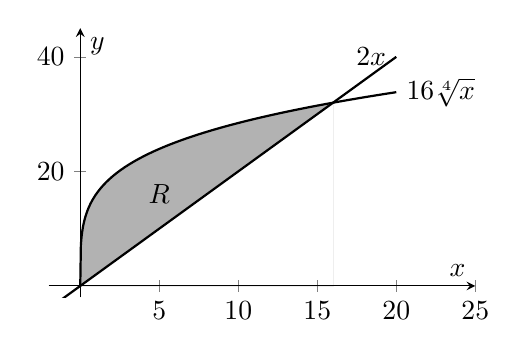
\begin{tikzpicture}
\begin{axis}[height=5cm, 
	width=7cm, 
	axis lines=middle,
	%axis line style={-latex}, 
	xmin=-2,xmax=25, 
	ymin=-2,ymax=45,
	%restrict y to domain=-1:10,
	%no markers, 
	xlabel={$x$},ylabel={$y$}, 
	%every axis x label/.append style={anchor=north}, 
	%every axis y label/.append style={anchor=east}, 
	area style,tension=0.08]
	
	\addplot+[domain=0:16,fill,black!30!white,samples=500]{16*x^(.25)} \closedcycle;
	\addplot+[domain=0:16,fill,white]{2*x} \closedcycle; 
	
	\addplot[domain=0:20,thick,smooth,samples=500]{16*x^(.25)} node[right] {$16\sqrt[4]{x}$}; 
	\addplot[domain=-5:20,thick] {2*x} node[left] {$2x$}; 	
	
	\node at (axis cs:5,16) {$R$};
\end{axis}
\end{tikzpicture}%
\end{minipage}\columnbreak

The intersections points: 
\begin{eqnarray*}
16x^{\nicefrac{1}{4}} & = & 2x\\
(2^{4}x^{\nicefrac{1}{4}})^{4} & = & (2x)^{4}\\
2^{16}x & = & 2^{4}x^{4}\\
2^{4}x(2^{12}-x^{3}) & = & 0\Rightarrow x=0\mbox{ and }x=16
\end{eqnarray*}

\end{multicols}

The general formula is: 
\[
\mbox{Volume}={\displaystyle \pi\int_{a}^{b}\underset{\overbrace{\mbox{{\tiny {top}}}}}{f(x)^{2}}-\underset{\overbrace{\mbox{{\tiny {bottom}}}}}{g(x)^{2}}\,dx\mbox{ (\textbf{NOT: }}{\displaystyle \int_{a}^{b}\left(f(x)-g(x)\right)^{2}\,dx}}\mbox{)}
\]

So we have, $\mbox{Volume}={\displaystyle \pi\int_{0}^{16}(}16x^{\nicefrac{1}{4}})^{2}-(2x)^{2}\,dx=\pi\left(\frac{512}{3}x^{\nicefrac{3}{2}}-\frac{4x^{3}}{3}\right)\Bigr|_{0}^{16}=\frac{16384}{3}\pi\mbox{ cubic units}$. 

\vfill
\end{document}
